% !Mode:: "TeX:UTF-8"
% !TEX program  = xelatex


Firstly, we should focus on the layout, you are using letter paper instead of A4 paper. And the line spacing you used is Chinese scheme. In addition, you should not indent in the first paragraph, which is Chinese scheme as well. The function of a paragraph indent is to mark a pause, setting the paragraph apart from what precedes it. If a paragraph is preceded by a title or subhead, the indent is superfluous and can therefore be omitted.

\begin{original}
    In this article, after\footnote{Maybe you can convert this sentence to ``we first introduce $\cdots$''} introducing some basic concepts of $\cdots$
\end{original}

\begin{original}
    And we will tell you when $n$\footnote{The context does not mention what $n$ is.} approaches infinity and the common radio less than 1, $\cdots$
    
    Because the article is short, we don't\footnote{Do not use ``don't''.} have content. But I think the section titles are clear enough.\footnote{Maybe you can delete this paragraph, since it is not helpful for content.}
\end{original}

\begin{original}
    \[
        S_n = \sum_{i=1}^{n}a_i = a_1+a_2+\ldots+a_n
    \]\footnote{Use \texttt{\backslash cdots} instead of \texttt{\backslash ldots}: $a_1+\cdots+a_n$.}
\end{original}

\begin{original}
    Next, we can define the sum\footnote{Note that the context should be consistent, convert ``sum'' to ``summation'' according to the title.} of the first $n$ terms in a squence.
\end{original}

\begin{original}
    We have $\frac{a_n}{a_{n-1}}=q$\footnote{Use \texttt{\backslash\$a\_n/a\_\{n-1\}\$} instead: $a_n/a_{n-1}$. Moreover, please pay attention to the processing between text and mathematical formulas.}, $\cdots$
\end{original}

\begin{original}
    If a sequence $\{a_n\}$ satisifies\footnote{Misspelling: satisfies.} the following condition: $\forall n=2,3,\ldots$\footnote{Do not use dots between formulas and text, which is easy to mislead the readers.} we have
\end{original}

\begin{original}
    And the equation (1)-(2)\footnote{Since you mentioned the Equation~(1)-(2) before, so you need to number the result and reference it here.} is called dislocation subtraction method.
\end{original}

\begin{original}
    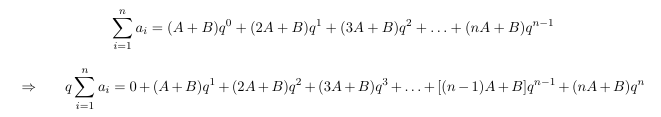
\includegraphics[width=\textwidth]{figures/geometric_progression-2}\footnote{If these two equations have relation, you should consider aligning the related parts. The following formulas need to pay attention to this proposal.}
\end{original}

\begin{original}
    \textbf{4.2 $\quad$ How does the formula change when $n\to\infty$ and $0<q<1$}\footnote{The title is too long, it is best not to include the formula.}
\end{original}

\begin{original}
    The author wishes to express his gratitude to Dr.\phantom{X}Zhang and Dr.\phantom{X}Wang\footnote{The space here is too big, maybe you should use \texttt{Dr.\backslash Wang} instead.} who $\cdots$
\end{original}

\begin{original}
    \begin{thebibliography}{9}
        \bibitem{C:1} Tang Tao. Mathematical Writing in English. 1st edition, 2013.
        \bibitem{C:2} https://baike.baidu.com/item/等比数列
        \bibitem{C:3} https://baike.baidu.com/item/棋盘麦粒问题/4764316?fr=aladdin
    \end{thebibliography}\footnote{The reference is not standardized and is not cited in the original text.}
\end{original}
